\documentclass[12pt]{article}
\usepackage[utf8]{inputenc}
\usepackage[italian]{babel}
\usepackage[T1]{fontenc}
\usepackage{natbib}
\usepackage{url}
\usepackage{amsmath}
\usepackage{graphicx}
\graphicspath{{images/}}
\usepackage{parskip}
\usepackage{fancyhdr}
\usepackage{vmargin}
\usepackage{hyperref}
\usepackage{xcolor} %per poter definire i colori e togliere i bordi colorati ai link
\usepackage{subcaption} %per raggruppare le figure
\usepackage{floatrow} %per caption laterale
\usepackage{lettrine} %per lettera grande all'inizio capitolo
\usepackage{gensymb} %per il simbolo °
\usepackage[font=footnotesize, labelfont=bf]{caption} %per modificare l'altezza del font dei caption
\captionsetup[sub]{font=scriptsize, labelfont=bf}
\captionsetup{margin=1cm}
\setmarginsrb{3 cm}{2.5 cm}{3 cm}{2.5 cm}{1 cm}{1.5 cm}{1 cm}{1.5 cm}

\title{Rilevazione superamento di corsia}				% Title
\author{Fabiola Polidoro \\ Davide Trenti}			% Author
\date{A.A. 2016/2017}											% Date

\makeatletter
\let\thetitle\@title
\let\theauthor\@author
\let\thedate\@date
\makeatother

%elimina i bordi colorati ai link
\hypersetup{
    colorlinks,
    linkcolor={black!50!black},
    citecolor={blue!50!black},
    urlcolor={blue!80!black}
}

\pagestyle{fancy}
\fancyhf{}
\rhead{Computer Vision}
\lhead{\thetitle}
%\fancyhead[R]{\rightmark}
%\fancyhead[L]{\thetitle}
\cfoot{\thepage}

\begin{document}

%%%%%%%%%%%%%%%%%%%%%%%%%%%%%%%%%%%%%%%%%%%%%%%%%%%%%%%%%%%%%%%%%%%%%%%%%%%%%%%%%%%%%%%%%

\begin{titlepage}
	\centering
    %\vspace*{0.5 cm}
    
\includegraphics[scale = 0.15]{polito.png}\\[1.0 cm]	% University Logo
    \textsc{\LARGE Politecnico di Torino}\\[1.5 cm]	% University Name
	\textsc{\Large Computer Vision}\\[0.1 cm]		% Course Code
	\textsc{\large 04ISFOV}\\[0.7 cm]				% Course Name
    \textsc{\large \bf TESINA}\\
	\rule{\linewidth}{0.2 mm} \\[0.4 cm]
	{ \huge \bfseries \thetitle}\\
	\rule{\linewidth}{0.2 mm} \\[1.5 cm]
	
	\begin{minipage}{0.4\textwidth}
		\begin{flushleft} \large
			\emph{Autori:}\\
			\theauthor
			\end{flushleft}
			\end{minipage}~
			\begin{minipage}{0.4\textwidth}
			\begin{flushright} \large
			\emph{Matricola:} \\
			231594 \\ 224714
            % Your Student Number
		\end{flushright}
	\end{minipage}\\[1.0 cm]
	
	{\large \emph{Docente:} \\
    prof. Luigi De Russis}\\[1.5cm]
	{\large \thedate}
 
	\vfill
	
\end{titlepage}

%%%%%%%%%%%%%%%%%%%%%%%%%%%%%%%%%%%%%%%%%%%%%%%%%%%%%%%%%%%%%%%%%%%%%%%%%%%%%%%%%%%%%%%%%

%%\tableofcontents
%%\pagebreak

%%%%%%%%%%%%%%%%%%%%%%%%%%%%%%%%%%%%%%%%%%%%%%%%%%%%%%%%%%%%%%%%%%%%%%%%%%%%%%%%%%%%%%%%%

\section{Introduzione}
\hspace{0.2 cm} Il \textit{lane departure warning system} è un meccanismo che avvisa il guidatore quando il suo veicolo sta uscendo dalla corsia di marcia, in modo da minimizzare gli incidenti dovuti ad errori, distrazioni o sonnolenza.
Il tipo più semplice di \textit{lane departure warning system} è quello che si limita ad avvertire il guidatore, in caso di superamento di corsia, mediante segnali visivi, uditivi oppure vibrazioni.\\
Il rilevamento delle strisce stradali avviene mediante una telecamera posta sul cruscotto della vettura e sensori laser e infrarossi montati davanti oppure sotto al veicolo.

\subsection{Obiettivo e requisiti della tesina}
\hspace{0.2 cm} L'obiettivo della tesina è quello di sviluppare un'applicazione desktop in grado di analizzare video ripresi da un'auto in movimento e di rilevare le due linee laterali della corsia, segnalando gli eventuali \textit{lane crossing}.
In particolare l'applicazione deve essere in grado di operare correttamente su video ripresi in condizioni di bel tempo sia di giorno che all'imbrunire oppure di notte su strade dotate di illuminazione. \\
I capitoli seguenti di questa relazione descriveranno i passi dello sviluppo e gli algoritmi utilizzati, in modo che questa tesina possa anche fungere come una sorta di documentazione per il programma stesso.

\subsection{Strumenti utilizzati}
\hspace{0.2 cm} Per lo sviluppo è stato utilizzato JavaFX che, oltre al Java, aggiunge JavaFX script e librerie grafiche per poter sviluppare interfacce utente.\\
Per gli algoritmi di computer vision invece è stata utilizzata la libreria OpenCV.

\newpage
\section{Implementazione software}
\subsection{Interfaccia grafica}
\hspace{0.2 cm} Il programma è dotato di un'interfaccia grafica composta principalmente da una barra dei menu, un'area in cui viene mostrato il video e un pannello sottostante contenente i controlli (\textit{stop}, \textit{play}, \textit{rewind}, \textit{fast forward}, \textit{slow}, \textit{next frame}, \textit{previous frame}) e informazioni come il nome del file, il numero di frame corrente e l'elapsed time.

Cliccando sulla voce ``\textit{Settings}'' nella barra del menu è possibile rendere visibile un pannello che permette di modificare quasi tutti i parametri relativi al riconoscimento delle linee di corsia e alla dimensione e posizionamento della \textit{region of interest} (ROI) su cui gli algoritmi lavorano.
Nella parte alta di tale pannello è presente un riquadro, che si adatta automaticamente all'aspect ratio del file video aperto, contornato da quattro slider che permettono di modificare la dimensione e la posizione della ROI, rappresentata come rettangolo azzurrino. Passando il mouse su ciascuno di questi slider, il contenuto del riquadro cambia temporaneamente per mostrare l'azione legata al comando.


\begin{figure}[htbp]
    \centering
    \begin{subfigure}[t]{0.32\textwidth}
        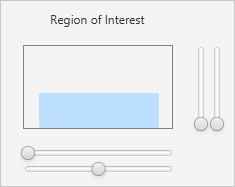
\includegraphics[width=\textwidth]{1.png}
        \caption{Posizione e dimensione corrente della ROI.}
	%\floatbox[{\capbeside\thisfloatsetup{capbesideposition={left,top},capbesidewidth=4cm}}]
	%{figure}[\FBwidth]
	%{\caption{A test figure with its caption side by side}}
	%{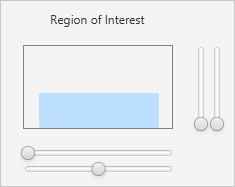
\includegraphics[width=\textwidth]{1.png}}
    \end{subfigure}
    \begin{subfigure}[t]{0.32\textwidth}
        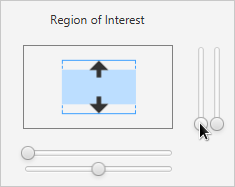
\includegraphics[width=\textwidth]{2.png}
        \caption{Aumenta/diminuisci l'altezza della ROI.}
    \end{subfigure}
    \begin{subfigure}[t]{0.32\textwidth}
        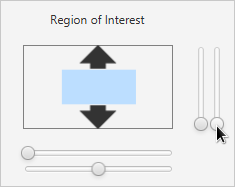
\includegraphics[width=\textwidth]{3.png}
        \caption{Sposta la ROI più in alto/basso.}
    \end{subfigure}
    \caption{Esempio di suggerimenti visivi relativi al posizionamento e alla dimensione verticali della \textit{region of interest}.}
\end{figure}


Degno di nota è anche l'elemento \texttt{TitledPane} ``Display'', che contiene una serie di checkbox che permettono di abilitare e disabilitare la visualizzazione sul video dei vari passi compiuti dall'algoritmo di \textit{lane detection}, come ad esempio i contorni, le strisce rilevate, quelle selezionate dall'algoritmo come facenti parte di una corsia e via dicendo.

\section{Lane detection}
\hspace{0.2 cm} Questo capitolo descrive come viene rilevata la corsia, supponendo che l'utente abbia già provveduto a selezionare un file video mediante il menu \texttt{File}$ \rightarrow $\texttt{Open} e ad eventualmente riposizionare la \textit{region of interest}.\\
È opportuno sottolineare che tutte le operazioni descritte nei paragrafi successivi vengono eseguite unicamente all'interno della ROI, pertanto occorre che essa sia posizionata in modo che il suo centro corrisponda al centro della corsia in cui si trova il veicolo e la parte superiore corrisponda all'orizzonte.

\subsection{Edge detection}
\hspace{0.2 cm} La prima azione eseguita su ciascun frame è la \textit{edge detection}, cioè il rilevamento dei bordi dell'immagine. Per questa operazione il frame deve essere convertito in scala di grigi mediante il metodo di OpenCV \texttt{cvtColor} con parametro \texttt{CV\char`_BGR2GRAY} e viene applicata una riduzione del rumore con il metodo \texttt{blur}.\\
In seguito viene applicato il metodo \texttt{Canny}, che dall'immagine in scala di grigi ne genera una binaria in cui il bianco rappresenta i bordi e il nero rappresenta tutto ciò che bordo non è.\\
La scelta del \texttt{Canny} rispetto ad altri metodi si è rivelata più efficace durante le prove.

Sia i parametri del \texttt{Canny} che quelli del \texttt{blur} hanno un valore di default preimpostato, modificabile manualmente tramite gli appositi slider nella sezione ``\textit{Canny}'' del pannello ``\textit{Settings}''.

\subsection{Line detection}
\hspace{0.2 cm} Una volta ottenuti i contorni dell'immagine si procede con l'individuazione delle linee mediante la trasformata di Hough probabilistica (\texttt{HoughLinesP}). Quest'ultima è stata scelta in quanto computazionalmente più efficiente rispetto alla trasformata di Hough semplice{\footnote{La trasformata di Hough semplice opera su ciascun punto dell'immagine, trovando la famiglia di linee passanti per esso, che dà luogo ad una sinusoide. Due punti distinti giacciono sulla stessa linea se le curve che li attraversano intersecano lo stesso piano. I parametri della linea individuata sono dati dalle coordinate polari $\rho$ e $\theta$ del punto in cui le curve si incontrano.\\ \hspace{0.2 cm}Per una spiegazione più dettagliata consultare la \href{http://docs.opencv.org/2.4/doc/tutorials/imgproc/imgtrans/hough_lines/hough_lines.html}{documentazione di OpenCV}.}}, dato che anzichè considerare tutti i punti di bordo dell'immagine, ne considera solo un sottoinsieme permettendo di ridurre il tempo di esecuzione.
I parametri del metodo \texttt{HoughLinesP} sono impostati ad un valore di default trovato empiricamente, ma sono anche modificabili manualmente dall'utente attraverso gli slider della sezione ``\textit{Hough properties}'' del pannello ``\textit{Settings}''.

\subsection{Scelta delle linee e disegno della corsia}
\hspace{0.2 cm} La trasformata di Hough probabilistica restituisce un array di linee, individuate dalle coordinate delle due estremità (x\ped1, y\ped1) e (x\ped2, y\ped2) ma, ai fini della \textit{lane detection}, non tutte sono utili. \\
Le linee vengono scelte in base ad alcuni parametri che possono essere calibrati tramite gli slider della sezione ``\textit{Lane constraints}'' del pannello ``\textit{Settings}'':
\begin{itemize}
\item pendenza (\textit{``slope''}) minima e massima. Una linea è considerata come probabile striscia stradale se la sua pendenza tende ad essere perpendicolare rispetto all'orizzonte ed è compresa in un intervallo impostato per default tra 10 e 90\degree. In questo modo vengono escluse le linee orizzontali o quasi orizzontali.
\item numero di linee candidate (``\textit{number of candidates}''). Per ciascuna linea, viene considerato l'estremo inferiore e vengono valutate la posizione e la distanza di quest'ultimo dal centro della \textit{region of interest}. In base alla posizione la linea è classificata come sinistra o destra e, in base alla distanza dell'estremo dal centro, è inserita in un \texttt{arrayList} ordinato, \texttt{leftList} oppure \texttt{rightList}, dopo essere stata estesa fino ai bordi della ROI. \\
Entrambi gli \texttt{arrayList} vengono potati, mantenendo solo le prime \textit{n} linee (``\textit{candidates}''), i cui estremi inferiori sono più vicini al centro.
\item angolo (\textit{``alpha''}) formato da una coppia di linee. Le linee presenti nei due \texttt{arrayList} \texttt{leftList} e \texttt{rightList} vengono combinate tra loro per formare coppie \texttt{<linea\char`_sinistra, linea\char`_destra>}. Tra esse vengono mantenute solo le coppie il cui angolo è compreso tra l'intervallo specificato dagli slider ``\textit{Min alpha}'' e ``\textit{Max alpha}'', che per default sono impostati rispettivamente a 65\degree e 120\degree.
\item distanza del punto di fuga delle linee dal centro della ROI (``\textit{Horizon radius}''). Una seconda potatura della lista di coppie candidate come corsia viene fatta considerando la distanza tra il punto di intersezione di ciascuna coppia e l'estremo superiore del centro della \textit{region of interest}.\\
Questo vincolo si è reso necessario per evitare che la presenza di frecce o altre scritte (ad esempio la lettera ``A'') sul manto stradale potesse trarre in inganno il programma e produrre un fastidioso \textit{flickering} della corsia evidenziata. Pertanto, solo le coppie la cui intersezione si trova entro un certo raggio dall'estremo superiore del centro della ROI vengono accettate come potenziale corsia.
\begin{figure}[htbp]
\centering
    \begin{subfigure}[b]{0.4\textwidth}
        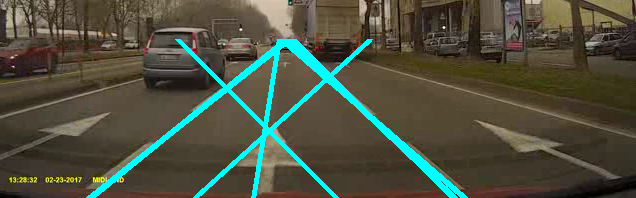
\includegraphics[width=\textwidth]{freccia.png}
    \end{subfigure}
    \begin{subfigure}[b]{0.4\textwidth}
        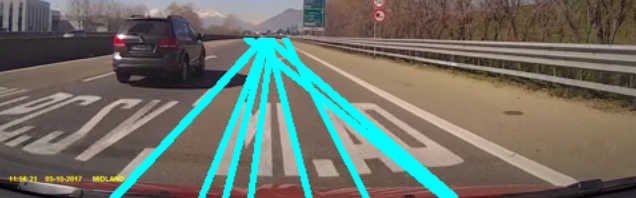
\includegraphics[width=\textwidth]{scritte.png}
    \end{subfigure}
\caption{Esempio di simboli e scritte che causano il \textit{flickering} della corsia.\\
Le linee azzurre rappresentano le coppie candidate.}
\end{figure}
\end{itemize}
Tra tutte le coppie, sarà scelta come candidata più probabile quella il cui \textit{alpha} si discosta meno da quello della coppia scelta nel frame precedente. Ciò permette di ridurre il \textit{flickering} della corsia quando il veicolo si trova su strade a più corsie.
\begin{figure}[htbp]
\centering
\begin{subfigure}[b]{0.4\textwidth}
        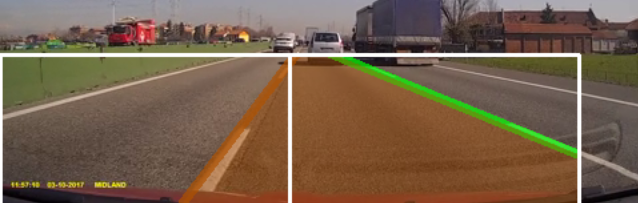
\includegraphics[width=\textwidth]{flickerCorsia1.png}
    \end{subfigure}
    \begin{subfigure}[b]{0.4\textwidth}
        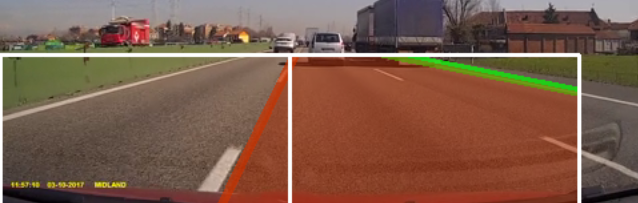
\includegraphics[width=\textwidth]{flickerCorsia2.png}
    \end{subfigure}
\caption{Esempio di flickering della corsia dovuto ad \textit{alpha} troppo diversi tra un frame e l'altro.}
\end{figure}

\hspace{0.2 cm} Prima di essere disegnata a video, la corsia deve rimanere stabile per un certo numero di frame, impostati dall'utente mediante lo slider "\textit{frames before showing lane}".\\
Se nessuna coppia di linee rispetta i vincoli imposti, viene disegnata l'ultima corsia valida rilevata nei frame precedenti. Il numero di tali frame è anch'esso impostabile tramite l'apposito slider "\textit{frames before hiding lane}". Se l'ultima corsia valida si trova nel passato, oltre il numero di frame specificati, nel frame corrente non viene più disegnata, in quanto si presuppone che il veicolo si trovi su un tratto di strada privo di segnaletica.

\subsection{Lane crossing}
\hspace{0.2 cm} Una volta individuate le linee che delimitano la corsia, viene calcolata la distanza tra il centro della \textit{region of interest} e l'estremità inferiore di ciascuna delle due strisce. Tali distanze, chiamate \texttt{leftDelta} e \texttt{rightDelta} vengono confrontate tra loro e, quella con valore minore, viene utilizzata per decidere il colore da assegnare al riempimento della corsia.
Il colore è definito come oggetto di tipo \texttt{Scalar}, il cui costruttore accetta tre parametri interi corrispondenti ai valori BGR, che in questo caso saranno impostati rispettivamente a:

\hspace{1.5 cm}(l) \texttt{(0, leftDelta, 255 - leftDelta)} per la striscia sinistra;

\hspace{1.5 cm}(r) \texttt{(0, rightDelta, 255 - rightDelta)} per quella destra.

\hspace{0.2 cm} Il lane crossing vero e proprio viene mostrato all'utente tramite il colore con cui viene riempita l'area compresa tra le due strisce, che può corrispondere, come già accennato, al caso (l) o (r), a seconda di chi tra \texttt{leftDelta} e \texttt{rightDelta} è minore.\\
Quando il veicolo si trova esattamente all'interno della corsia il colore è verde e, man mano che si avvicina alla linea di mezzeria, il colore sfuma via via verso l'arancione fino a raggiungere il rosso quando il veicolo si trova a cavallo della striscia. \\
\begin{figure}[htbp]
\centering
    \begin{subfigure}[b]{0.24\textwidth}
        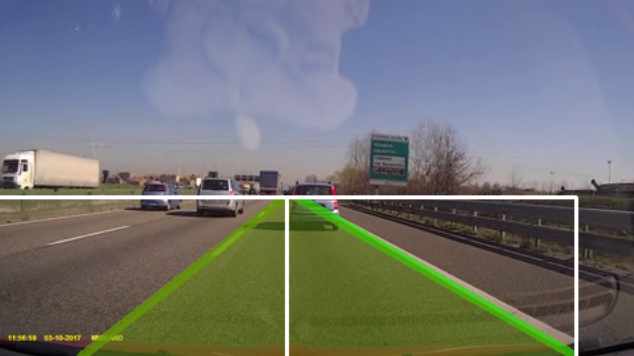
\includegraphics[width=\textwidth]{cross_1.png}
    \end{subfigure}
    \begin{subfigure}[b]{0.24\textwidth}
        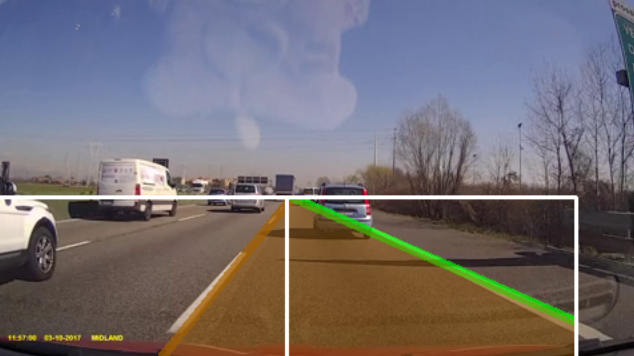
\includegraphics[width=\textwidth]{cross_2.png}
    \end{subfigure}
    \begin{subfigure}[b]{0.24\textwidth}
        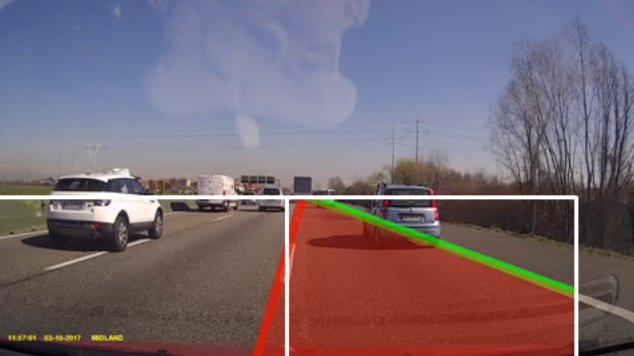
\includegraphics[width=\textwidth]{cross_3.png}
    \end{subfigure}
    \begin{subfigure}[b]{0.24\textwidth}
        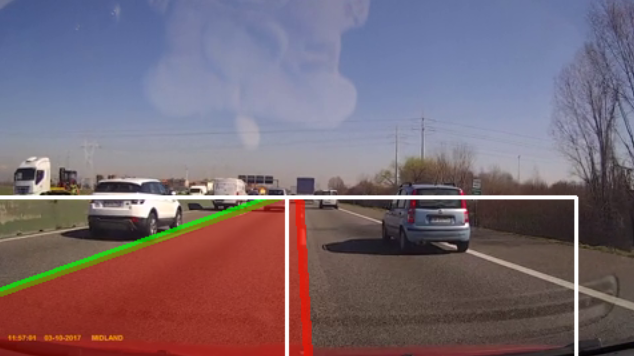
\includegraphics[width=\textwidth]{cross_4.png}
    \end{subfigure}
\caption{\textit{Lane crossing} verso sinistra evidenziato con i colori.}
\end{figure}

\subsection{Risultati}
\hspace{0.2 cm} L'algoritmo è stato testato principalmente con video girati con la nostra \textit{dash cam} su strade urbane, extraurbane e tangenziali, nelle condizioni richieste dai requisiti della tesina, pertanto i parametri di default sono stati impostati per garantire il miglior funzionamento con essi.\\
In aggiunta, sono stati usati anche filmati forniti dal docente per verificare l'adattività dei parametri a video girati con dispositivi diversi dal nostro.\\
Di seguito sono riportati i commenti su ciascun file.
\begin{itemize}
\item \texttt{2756\char`_giorno.avi}. La \textit{lane detection} funziona correttamente per quasi tutta la durata del video: per alcuni istanti la corsia non viene rilevata quando il veicolo si trova in prossimità dell'uscita dalla galleria urbana e durante il lane crossing in prossimità del semaforo. Ciò è molto probabilmente dovuto al repentino cambio di illuminazione dell'intera scena, per il primo caso, e alla eccessiva vicinanza del nostro veicolo all'auto ferma al rosso.
\item \texttt{2873\char`_giorno.avi}. Anche in questo caso l'algoritmo non dà particolari problemi per la maggior parte del tempo. In alcuni tratti di curva, la corsia non viene rilevata a causa di angoli \textit{``alpha''} troppo grandi rispetto a quelli impostati di default. Aumentando il parametro \textit{``max alpha''}, si verifica un fastidioso ``\textit{flickering} di corsia'' appena il veicolo giunge su strada a tre corsie, pertanto si è preferito avere questi vuoti in curva piuttosto che rilevamenti sbagliati sui rettilinei.\\
Oltre agli sfarfallii dovuti alla segnaletica stradale, si ottengono effetti simili anche quando il veicolo passa accanto a TIR o bus, che proiettano un'ombra lunga sulla carreggiata.
%%%%figura del tir
\begin{figure}[htbp]
\centering
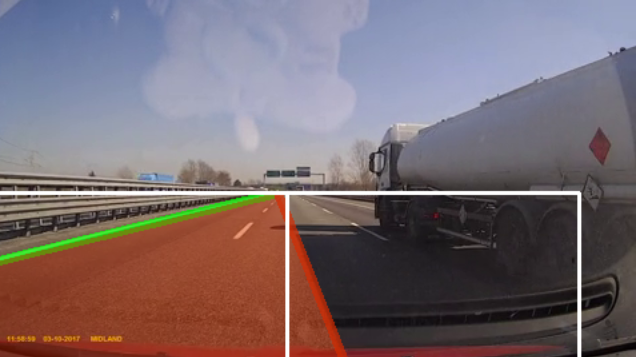
\includegraphics[scale=0.5]{tir.png}
\caption{Rilevamento errato della corsia dovuto all'ombra di un TIR.}
\end{figure}

\item \texttt{2980\char`_notte.avi}. Questo filmato ripercorre, di notte, lo stesso tratto di strada del filmato \texttt{2873\char`_giorno.avi} e, fino all'immissione nella tangenziale vera e propria, la corsia viene sempre rilevata in modo corretto, a parte gli sfarfallii dovuti alla segnaletica stradale già descritti in precedenza.\\
L'algoritmo incontra difficoltà nel rilevare sempre la corsia quando l'illuminazione stradale è assente (tratti extraurbani), anche se nel complesso le prestazioni si possono considerare accettabili.
\item \texttt{2796\char`_imbrunire.avi} e \texttt{2797\char`_imbrunire.avi}. Per entrambi i filmati l'algoritmo funziona perfettamente per tutta la durata, nonostante nel secondo video l'illuminazione stradale sia abbastanza scarsa. Occasionalmente si verificano piccoli sfarfallii dovuti a segni di frenata sull'asfalto che però non invalidano il rilevamento della corsia.
\item \texttt{V4\char`_highway.mp4}, \texttt{V3\char`_cross1.mp4} e \texttt{V3\char`_cross2.mp4}. I parametri di default si adattano bene ai tre video, nonostante siano comunque presenti sfarfallii di corsia dovuti a segni di frenata sull'asfalto, molto più evidenti rispetto al video \texttt{2796\char`_imbrunire.avi} poichè l'asfalto ha un colore molto più chiaro.
\item \texttt{V2\char`_highway.mp4}. La \textit{lane detection} in questo filmato dà pessimi risultati con i parametri di default, in quanto la corsia non viene mai rilevata. Impostando il parametro \textit{``Max alpha''} a 150 si ottiene un risultato accettabile anche se con frequenti sfarfallii di corsia.
\item \texttt{V1\char`_regular.mp4}. Anche con questo video i parametri di default non vanno bene, poichè la corsia non viene rilevata in prossimità delle curve. Queste ultime sono molto strette e causano un eccessivo spostamento del punto di incontro delle linee destra e sinistra dal punto centrale superiore della \textit{region of interest}.\\
In questo caso, per ottenere un rilevamento corretto, oltre che impostare il parametro \textit{``Max alpha''} a 150, occorre anche modificare il parametro \textit{``Horizon variance''} impostandolo a 90.
\end{itemize}


\newpage
\section{Migliorie}
\hspace{0.2cm} Nella sua versione attuale il programma può essere adattato manualmente per l'utilizzo con filmati molto diversi tra loro in termini di qualità video ed illuminazione, tuttavia sarebbe possibile migliorarlo ulteriormente implementando le seguenti funzionalità:
\begin{itemize}
\item adattività automatica dei parametri (ad esempio Canny, Blur, trasformata di Hough) in base alla risoluzione del video, alla qualità e all'illuminazione;
\item riconoscimento automatico del punto di fuga e ridimensionamento automatico della \textit{region of interest} in base alla larghezza della corsia, così che l'algoritmo di \textit{lane detection} si comporti correttamente con qualsiasi tipo di curva e in presenza di salite e discese ripide che fanno variare l'altezza dell'orizzonte;
\item gestione e rimozione di crepe e segni di frenata sull'asfalto, tramite filtraggio dei colori prima dell'applicazione del Canny;
\item evidenziazione della corsia con un contorno preciso e non triangolare, mediante suddivisione della \textit{region of interest} in sub-ROI, o, in alternativa, riempimento con gradiente di trasparenza verticale;
\item estensione del supporto a filmati ad alta risoluzione: l'applicazione attuale non è in grado di riprodurre tali video ad un frame rate accettabile, infatti si è reso necessario ridurre di quattro volte i filmati full HD ripresi con la nostra \textit{dash cam}.
\end{itemize}

\hspace{0.2cm}Risultati molto migliori possono essere ottenuti con tecniche che utilizzano cambi di prospettiva (\textit{Bird's eye view}) per rendere parallele tra loro le linee di corsia e permetterne una manipolazione più accurata e \textit{machine learning} per riconoscere la segnaletica sull'asfalto e ridurre gli errori nel riconoscimento delle corsie.

\end{document}
